

\tikzset{every picture/.style={line width=0.75pt}} %set default line width to 0.75pt        

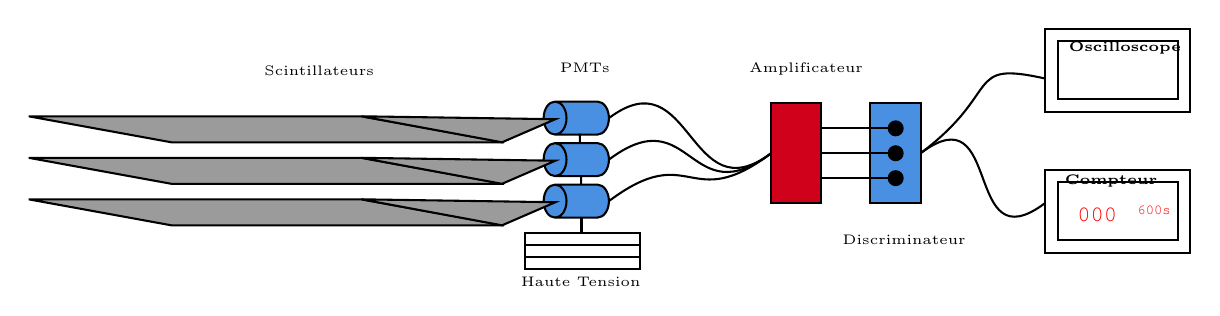
\begin{tikzpicture}[x=0.75pt,y=0.75pt,yscale=-1,xscale=1]
%uncomment if require: \path (0,300); %set diagram left start at 0, and has height of 300

%Shape: Parallelogram [id:dp6153094668241826] 
\draw  [fill={rgb, 255:red, 155; green, 155; blue, 155 }  ,fill opacity=1 ][line width=0.75]  (234.63,54.2) -- (74.3,54.2) -- (143.01,66.72) -- (303.34,66.72) -- cycle ;
%Flowchart: Direct Access Storage [id:dp057480924744088946] 
\draw  [fill={rgb, 255:red, 74; green, 144; blue, 226 }  ,fill opacity=1 ][line width=0.75]  (327.9,63) -- (348.34,63) .. controls (351.38,63) and (353.84,59.45) .. (353.84,55.06) .. controls (353.84,50.67) and (351.38,47.12) .. (348.34,47.12) -- (327.9,47.12)(322.4,55.06) .. controls (322.4,59.45) and (324.86,63) .. (327.9,63) .. controls (330.94,63) and (333.4,59.45) .. (333.4,55.06) .. controls (333.4,50.67) and (330.94,47.12) .. (327.9,47.12) .. controls (324.86,47.12) and (322.4,50.67) .. (322.4,55.06) ;
%Shape: Triangle [id:dp281161219892323] 
\draw  [fill={rgb, 255:red, 155; green, 155; blue, 155 }  ,fill opacity=1 ][line width=0.75]  (328.02,55.6) -- (302.35,66.73) -- (234.63,54.2) -- cycle ;

%Shape: Parallelogram [id:dp9101804879233704] 
\draw  [fill={rgb, 255:red, 155; green, 155; blue, 155 }  ,fill opacity=1 ] (234.63,74.2) -- (74.3,74.2) -- (143.01,86.72) -- (303.34,86.72) -- cycle ;
%Flowchart: Direct Access Storage [id:dp015646766055150918] 
\draw  [fill={rgb, 255:red, 74; green, 144; blue, 226 }  ,fill opacity=1 ] (327.9,83) -- (348.34,83) .. controls (351.38,83) and (353.84,79.45) .. (353.84,75.06) .. controls (353.84,70.67) and (351.38,67.12) .. (348.34,67.12) -- (327.9,67.12)(322.4,75.06) .. controls (322.4,79.45) and (324.86,83) .. (327.9,83) .. controls (330.94,83) and (333.4,79.45) .. (333.4,75.06) .. controls (333.4,70.67) and (330.94,67.12) .. (327.9,67.12) .. controls (324.86,67.12) and (322.4,70.67) .. (322.4,75.06) ;
%Shape: Triangle [id:dp42632878589040457] 
\draw  [fill={rgb, 255:red, 155; green, 155; blue, 155 }  ,fill opacity=1 ] (328.02,75.6) -- (302.35,86.73) -- (234.63,74.2) -- cycle ;

%Shape: Parallelogram [id:dp08291359315510605] 
\draw  [fill={rgb, 255:red, 155; green, 155; blue, 155 }  ,fill opacity=1 ] (234.63,94.2) -- (74.3,94.2) -- (143.01,106.72) -- (303.34,106.72) -- cycle ;
%Flowchart: Direct Access Storage [id:dp39415762621948935] 
\draw  [fill={rgb, 255:red, 74; green, 144; blue, 226 }  ,fill opacity=1 ] (327.9,103) -- (348.34,103) .. controls (351.38,103) and (353.84,99.45) .. (353.84,95.06) .. controls (353.84,90.67) and (351.38,87.12) .. (348.34,87.12) -- (327.9,87.12)(322.4,95.06) .. controls (322.4,99.45) and (324.86,103) .. (327.9,103) .. controls (330.94,103) and (333.4,99.45) .. (333.4,95.06) .. controls (333.4,90.67) and (330.94,87.12) .. (327.9,87.12) .. controls (324.86,87.12) and (322.4,90.67) .. (322.4,95.06) ;
%Shape: Triangle [id:dp44810110314081986] 
\draw  [fill={rgb, 255:red, 155; green, 155; blue, 155 }  ,fill opacity=1 ] (328.02,95.6) -- (302.35,106.73) -- (234.63,94.2) -- cycle ;

%Curve Lines [id:da8784603980762927] 
\draw    (353.84,55.06) .. controls (393.84,25.06) and (392,102) .. (432,72) ;
%Curve Lines [id:da9313823595606255] 
\draw    (353.84,75.06) .. controls (393.84,45.06) and (392,102) .. (432,72) ;
%Curve Lines [id:da24872657353422778] 
\draw    (353.84,95.06) .. controls (393.84,65.06) and (392,102) .. (432,72) ;
%Shape: Rectangle [id:dp7955377352395961] 
\draw  [fill={rgb, 255:red, 208; green, 2; blue, 27 }  ,fill opacity=1 ] (432,48) -- (456.24,48) -- (456.24,96) -- (432,96) -- cycle ;
%Shape: Frame [id:dp790746320543737] 
\draw   (564,12) -- (634,12) -- (634,52) -- (564,52) -- cycle(628,18) -- (570,18) -- (570,46) -- (628,46) -- cycle ;
%Shape: Rectangle [id:dp8336691747772105] 
\draw   (313.2,116.11) -- (368.64,116.11) -- (368.64,121.89) -- (313.2,121.89) -- cycle ;
%Shape: Rectangle [id:dp6493800754350441] 
\draw   (313.2,121.89) -- (368.64,121.89) -- (368.64,127.68) -- (313.2,127.68) -- cycle ;
%Shape: Rectangle [id:dp7269506258160386] 
\draw   (313.2,110.32) -- (368.64,110.32) -- (368.64,116.11) -- (313.2,116.11) -- cycle ;

%Straight Lines [id:da6829845507956613] 
\draw    (340.64,102.64) -- (340.64,110.2) ;
%Straight Lines [id:da5330000370742687] 
\draw    (340.4,82.89) -- (340.49,87.27) ;
%Straight Lines [id:da5174947670175065] 
\draw    (339.78,62.58) -- (339.87,66.97) ;
%Shape: Rectangle [id:dp7820496204409214] 
\draw  [fill={rgb, 255:red, 74; green, 144; blue, 226 }  ,fill opacity=1 ] (479.76,48) -- (504,48) -- (504,96) -- (479.76,96) -- cycle ;
%Shape: Frame [id:dp44415473016363605] 
\draw   (564,80) -- (634,80) -- (634,120) -- (564,120) -- cycle(628,86) -- (570,86) -- (570,114) -- (628,114) -- cycle ;
%Curve Lines [id:da7027674246282678] 
\draw    (504,72) .. controls (544,42) and (524.71,27.29) .. (564,36) ;
%Curve Lines [id:da161234971098009] 
\draw    (504,72) .. controls (544,42) and (524,126) .. (564,96) ;
%Straight Lines [id:da2592906745330712] 
\draw    (456,60) -- (492,60) ;
\draw [shift={(492,60)}, rotate = 0] [color={rgb, 255:red, 0; green, 0; blue, 0 }  ][fill={rgb, 255:red, 0; green, 0; blue, 0 }  ][line width=0.75]      (0, 0) circle [x radius= 3.35, y radius= 3.35]   ;
%Straight Lines [id:da4896356965331372] 
\draw    (456,72) -- (492,72) ;
\draw [shift={(492,72)}, rotate = 0] [color={rgb, 255:red, 0; green, 0; blue, 0 }  ][fill={rgb, 255:red, 0; green, 0; blue, 0 }  ][line width=0.75]      (0, 0) circle [x radius= 3.35, y radius= 3.35]   ;
%Straight Lines [id:da963095590048375] 
\draw    (456,84) -- (492,84) ;
\draw [shift={(492,84)}, rotate = 0] [color={rgb, 255:red, 0; green, 0; blue, 0 }  ][fill={rgb, 255:red, 0; green, 0; blue, 0 }  ][line width=0.75]      (0, 0) circle [x radius= 3.35, y radius= 3.35]   ;

% Text Node
\draw (574,17) node [anchor=north west][inner sep=0.75pt]   [align=left] {{\tiny \textbf{Oscilloscope}}};
% Text Node
\draw (420,27) node [anchor=north west][inner sep=0.75pt]   [align=left] {{\tiny Amplificateur}};
% Text Node
\draw (328.8,27) node [anchor=north west][inner sep=0.75pt]   [align=left] {{\tiny PMTs}};
% Text Node
\draw (186.4,28.2) node [anchor=north west][inner sep=0.75pt]   [align=left] {{\tiny Scintillateurs}};
% Text Node
\draw (310,130) node [anchor=north west][inner sep=0.75pt]   [align=left] {{\tiny Haute Tension}};
% Text Node
\draw (465,110) node [anchor=north west][inner sep=0.75pt]   [align=left] {{\tiny Discriminateur}};
% Text Node
\draw (578,97) node [anchor=north west][inner sep=0.75pt]  [font=\footnotesize] [align=left] {{\fontfamily{pcr}\selectfont {\footnotesize \textcolor[rgb]{1,0,0}{000}}}};
% Text Node
\draw (607,96) node [anchor=north west][inner sep=0.75pt]  [font=\footnotesize] [align=left] {{\fontfamily{pcr}\selectfont {\tiny \textcolor[rgb]{1,0,0}{600s}}}};
% Text Node
\draw (572,81) node [anchor=north west][inner sep=0.75pt]   [align=left] {{\tiny \textbf{Compteur}}};


\end{tikzpicture}
